\clearpage
\subsection*{MATLAB time histories}
Parameters P1--P4 follow Homework 1. The two pendulum lengths are $l_1$ and $l_2$; for P4, $l_1=1$, $l_2=0.5$.

State order: $x=[y,\theta_1,\theta_2,\dot y,\dot\theta_1,\dot\theta_2]^T$. Both models start from the same physical state $x(0)=x^e+z(0)$, with $u=0$. Plots show deviations $z=x-x^e$; angles are in degrees and are not wrapped.

For Exercise 7(b), $z(0)=[0,-\alpha,+\alpha,0,0,0]^T$ (angular entries converted from degrees to radians). L7 uses $\alpha=0,1,10,90,180$ deg and L8 uses $\alpha=1$ deg. L7 is simulated for 30 s and L8 for 5 s.

Nonlinear simulation: \texttt{ode45}, relative tolerance $10^{-10}$, absolute tolerance $10^{-12}$, maximum step 0.02 s. Linear responses use the matrix exponential.
\clearpage
\subsection*{\texttt{ex7\_L7\_000deg}}
Initial deviation $z(0)$ (radians for angles, SI units otherwise):
\begin{center}\scriptsize\texttt{[0, -0, 0, 0, 0, 0]}\end{center}
$x^e=[0,0,0,0,0,0]^T$, $x(0)=x^e+z(0)$.
\begin{figure}[!ht]
\centering
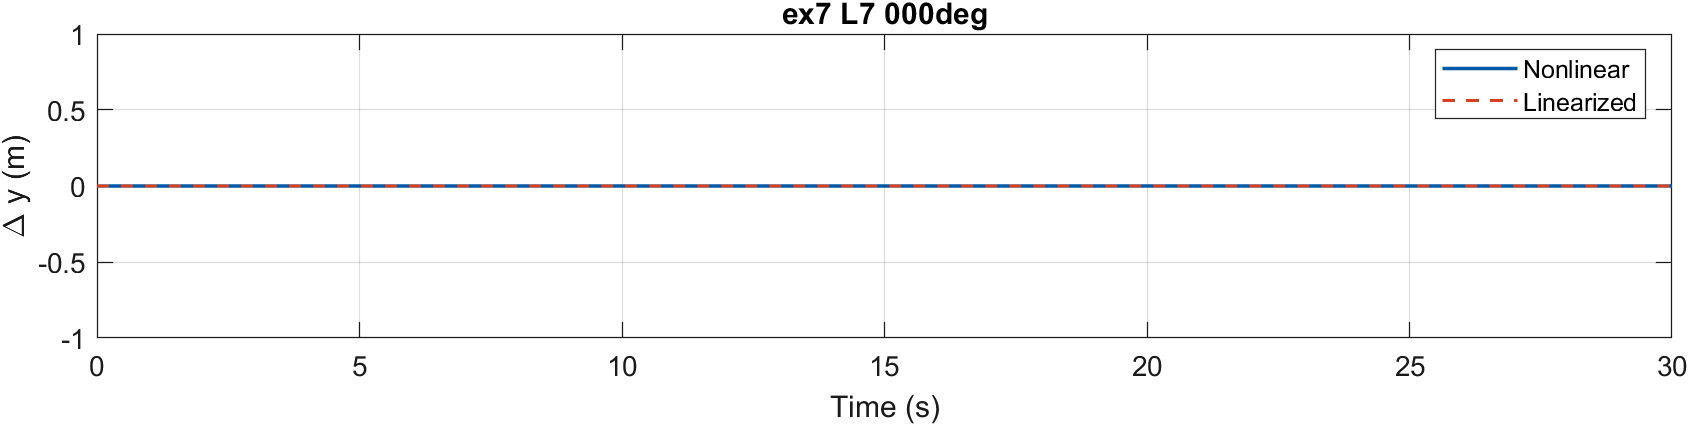
\includegraphics[width=0.94\linewidth]{figures/ex7_L7_000deg_y.png}
\caption{$\Delta y$: nonlinear and linearized time histories.}
\end{figure}
\begin{figure}[!ht]
\centering
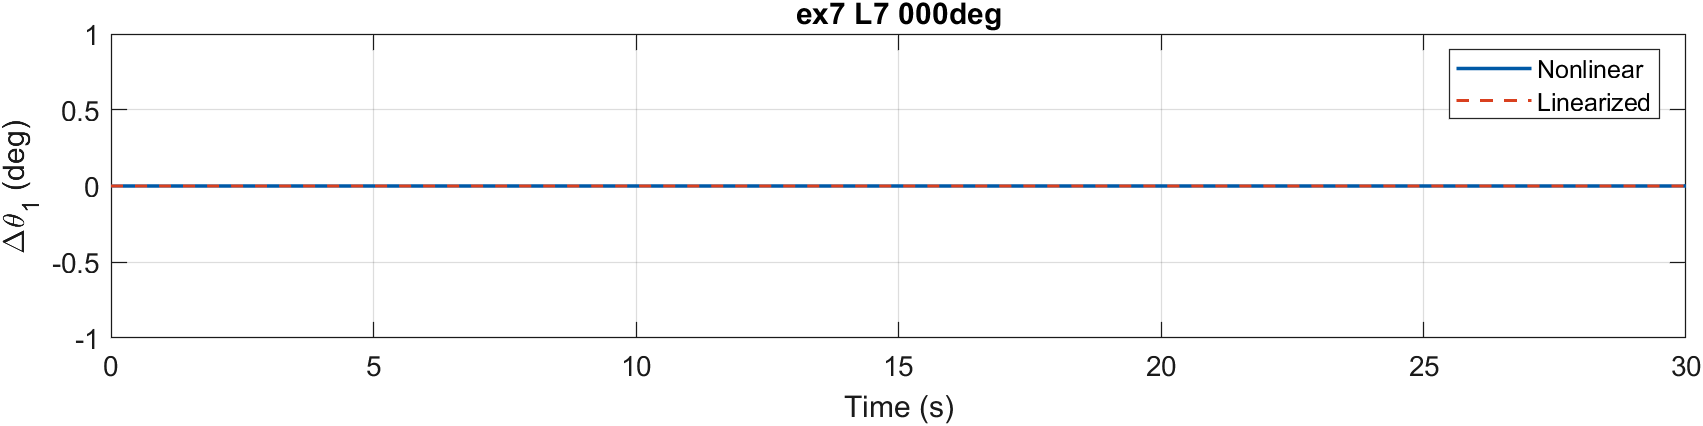
\includegraphics[width=0.94\linewidth]{figures/ex7_L7_000deg_theta1.png}
\caption{$\Delta\theta_1$: nonlinear and linearized time histories.}
\end{figure}
\begin{figure}[!ht]
\centering
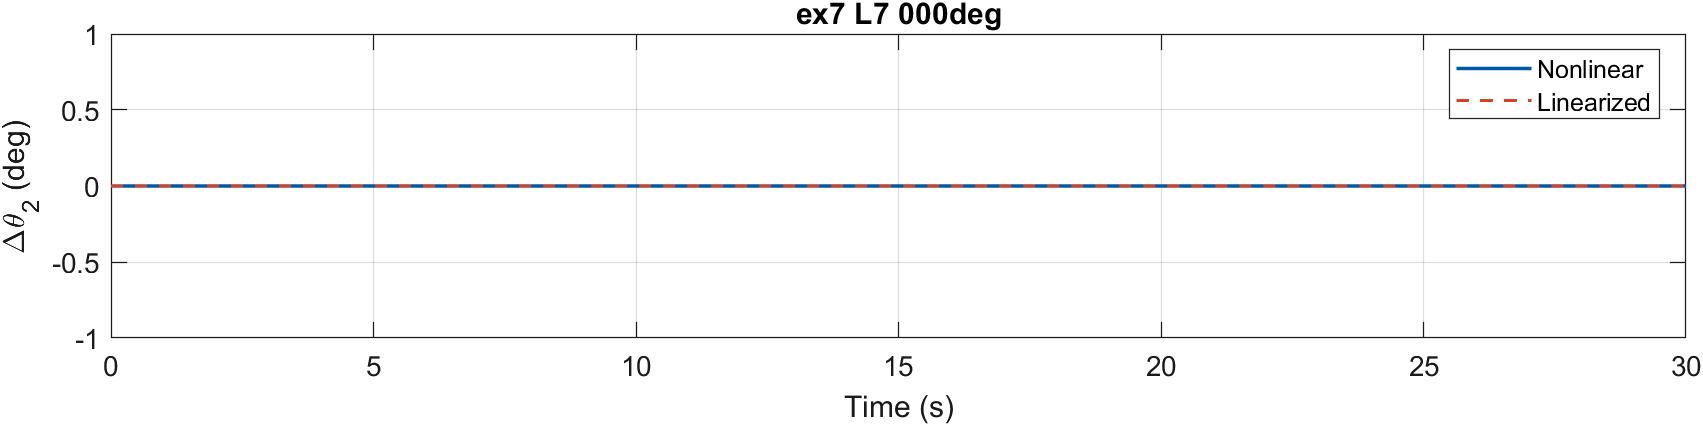
\includegraphics[width=0.94\linewidth]{figures/ex7_L7_000deg_theta2.png}
\caption{$\Delta\theta_2$: nonlinear and linearized time histories.}
\end{figure}

\clearpage
\subsection*{\texttt{ex7\_L7\_001deg}}
Initial deviation $z(0)$ (radians for angles, SI units otherwise):
\begin{center}\scriptsize\texttt{[0, -0.01745329, 0.01745329, 0, 0, 0]}\end{center}
$x^e=[0,0,0,0,0,0]^T$, $x(0)=x^e+z(0)$.
\begin{figure}[!ht]
\centering
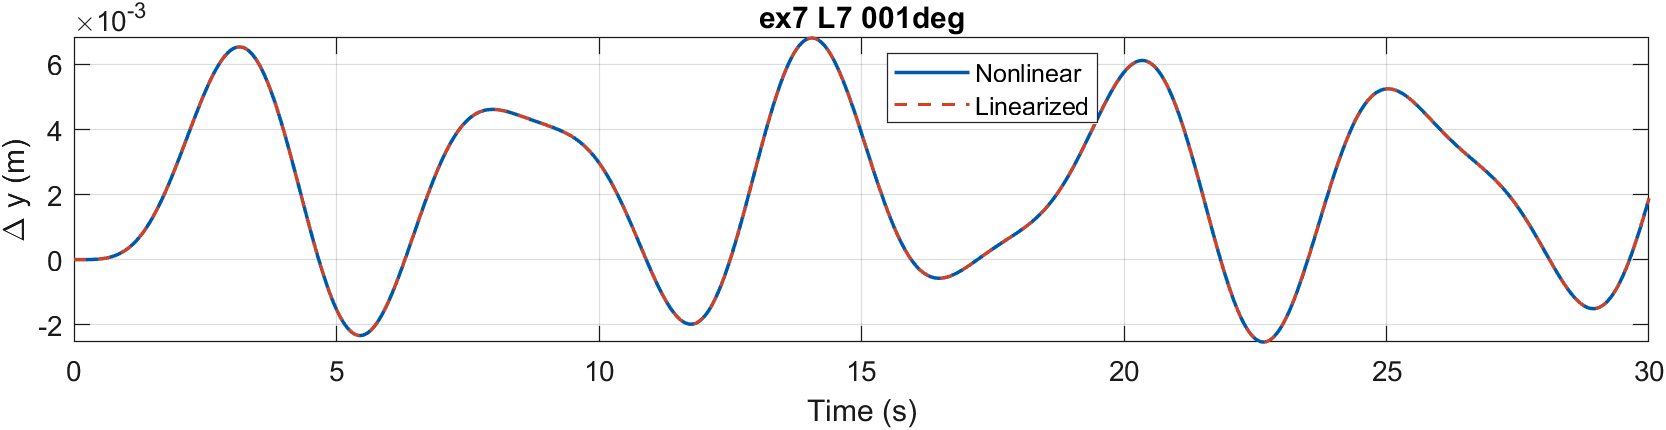
\includegraphics[width=0.94\linewidth]{figures/ex7_L7_001deg_y.png}
\caption{$\Delta y$: nonlinear and linearized time histories.}
\end{figure}
\begin{figure}[!ht]
\centering
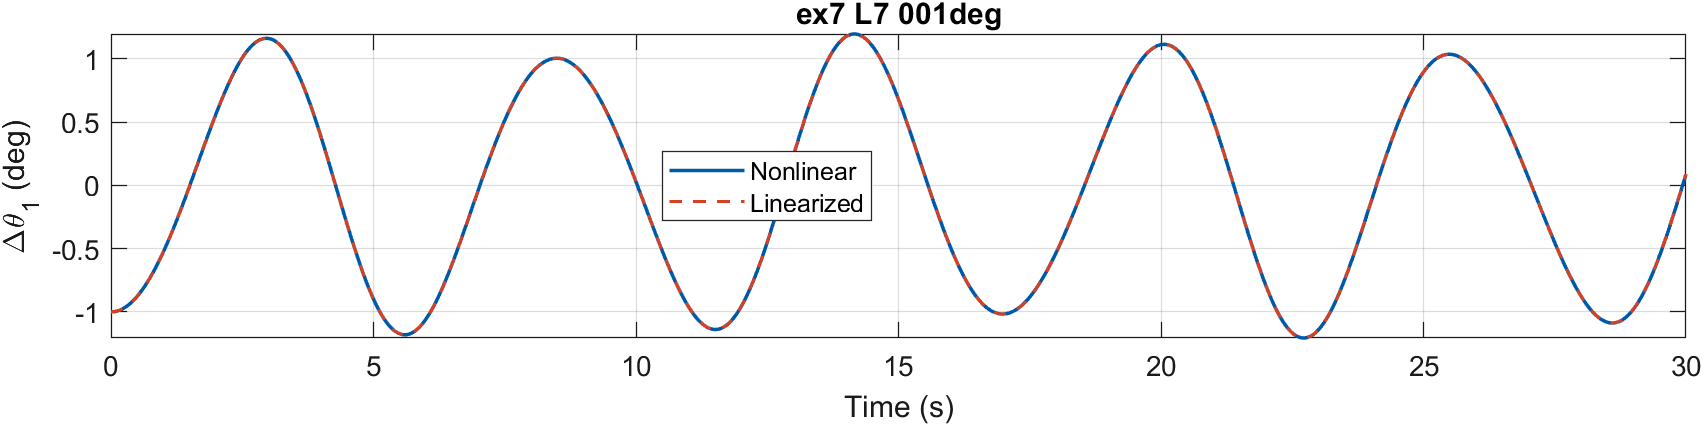
\includegraphics[width=0.94\linewidth]{figures/ex7_L7_001deg_theta1.png}
\caption{$\Delta\theta_1$: nonlinear and linearized time histories.}
\end{figure}
\begin{figure}[!ht]
\centering
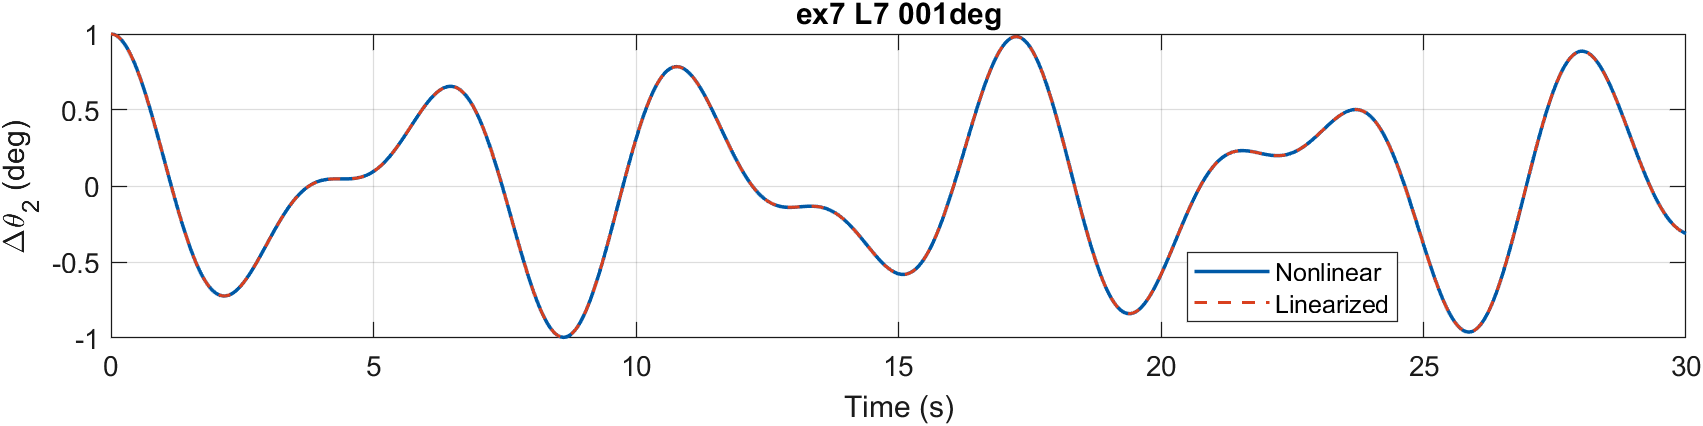
\includegraphics[width=0.94\linewidth]{figures/ex7_L7_001deg_theta2.png}
\caption{$\Delta\theta_2$: nonlinear and linearized time histories.}
\end{figure}

\clearpage
\subsubsection*{L7: $\pm10^\circ$}
Initial deviation $z(0)$ (radians for angles, SI units otherwise):
\begin{center}\scriptsize\texttt{[0, -0.1745329, 0.1745329, 0, 0, 0]}\end{center}
$x^e=[0,0,0,0,0,0]^T$, $x(0)=x^e+z(0)$.
\begin{figure}[!ht]
\centering
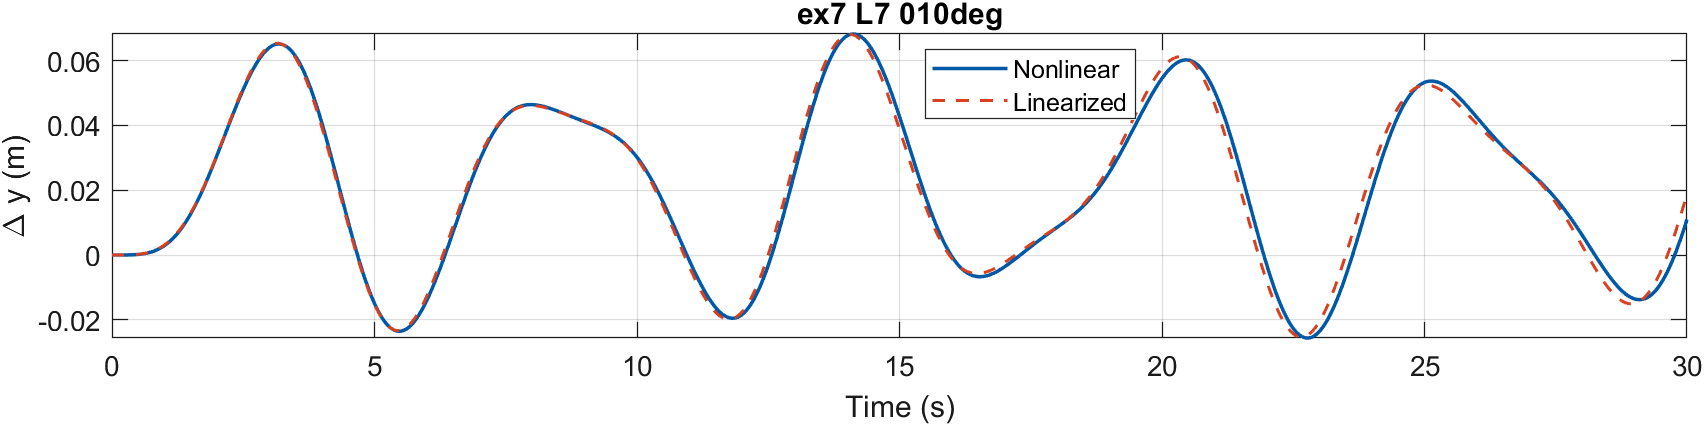
\includegraphics[width=0.94\linewidth]{figures/ex7_L7_010deg_y.png}
\caption{$\Delta y$: nonlinear and linearized time histories.}
\end{figure}
\begin{figure}[!ht]
\centering
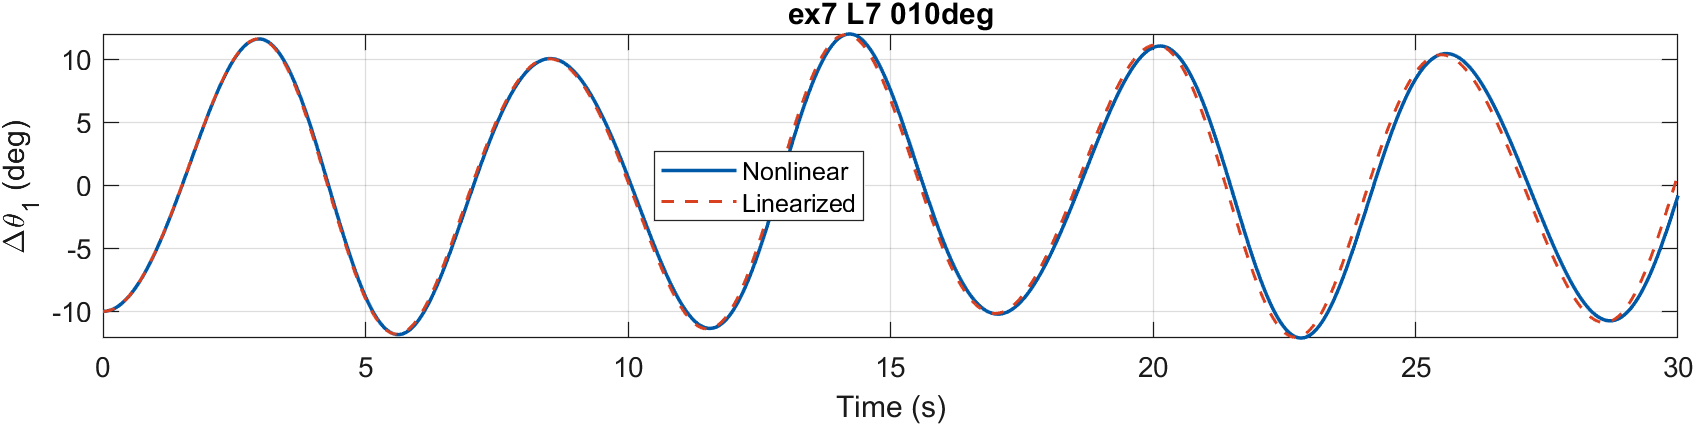
\includegraphics[width=0.94\linewidth]{figures/ex7_L7_010deg_theta1.png}
\caption{$\Delta\theta_1$: nonlinear and linearized time histories.}
\end{figure}
\begin{figure}[!ht]
\centering
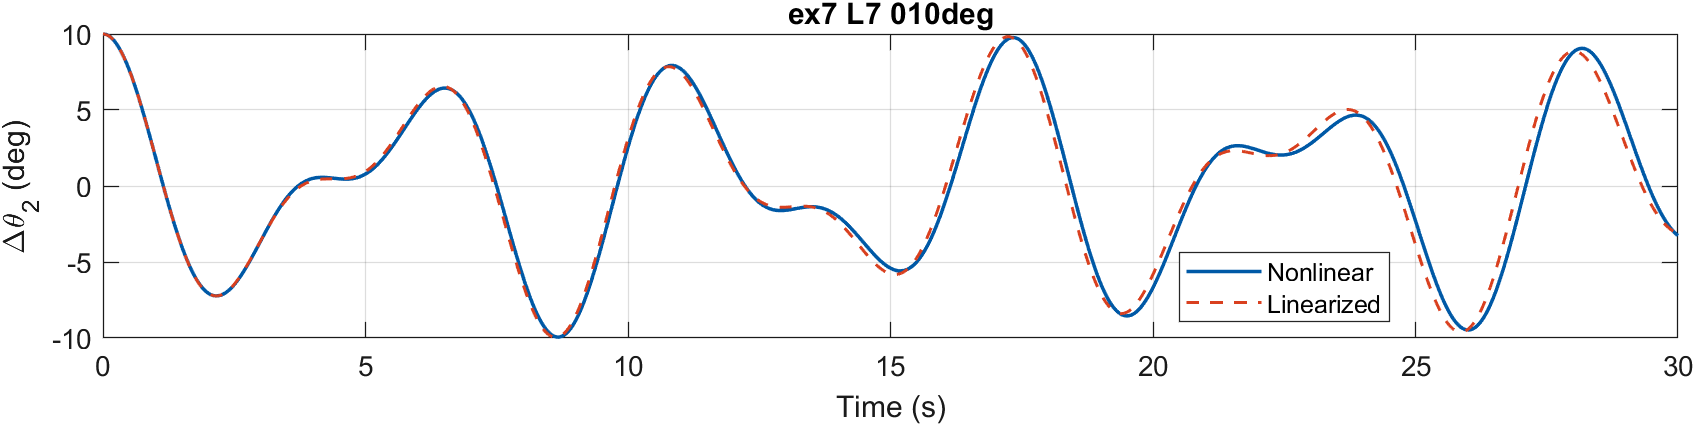
\includegraphics[width=0.94\linewidth]{figures/ex7_L7_010deg_theta2.png}
\caption{$\Delta\theta_2$: nonlinear and linearized time histories.}
\end{figure}
\clearpage
\textbf{MATLAB code for L7, $\pm10^\circ$:}
The following case-specific block uses the common local functions \texttt{simulate\_case} and \texttt{export\_case} listed in the source appendix.
\begin{lstlisting}
p = [2 1 1 1 0.5 1]; % [m0 m1 m2 l1 l2 g]
model = cart_pendulum_model(p, 1);
alpha = 10; % degrees
z0 = [0; -deg2rad(alpha); deg2rad(alpha); 0; 0; 0];
options = odeset('RelTol',1e-10,'AbsTol',1e-12,'MaxStep',0.02);
r = simulate_case(model, z0, 30, 'ex7_L7_010deg', options);
export_case(r, outputDir, rootDir);
\end{lstlisting}

\clearpage
\subsubsection*{L7: $\pm90^\circ$}
Initial deviation $z(0)$ (radians for angles, SI units otherwise):
\begin{center}\scriptsize\texttt{[0, -1.570796, 1.570796, 0, 0, 0]}\end{center}
$x^e=[0,0,0,0,0,0]^T$, $x(0)=x^e+z(0)$.
\begin{figure}[!ht]
\centering
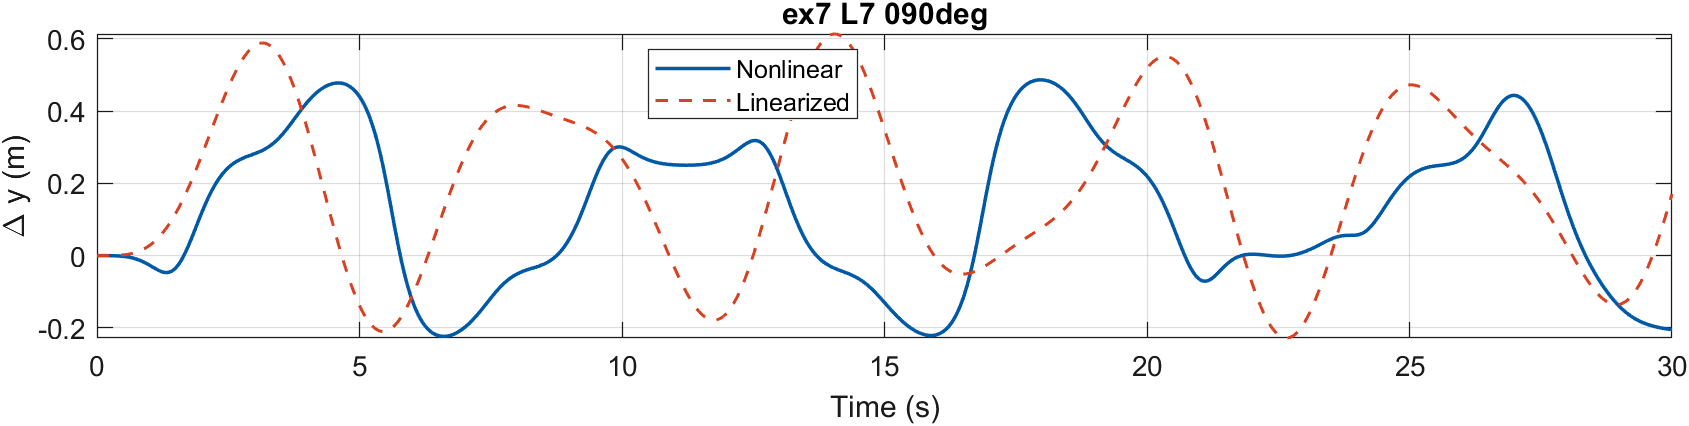
\includegraphics[width=0.94\linewidth]{figures/ex7_L7_090deg_y.png}
\caption{$\Delta y$: nonlinear and linearized time histories.}
\end{figure}
\begin{figure}[!ht]
\centering
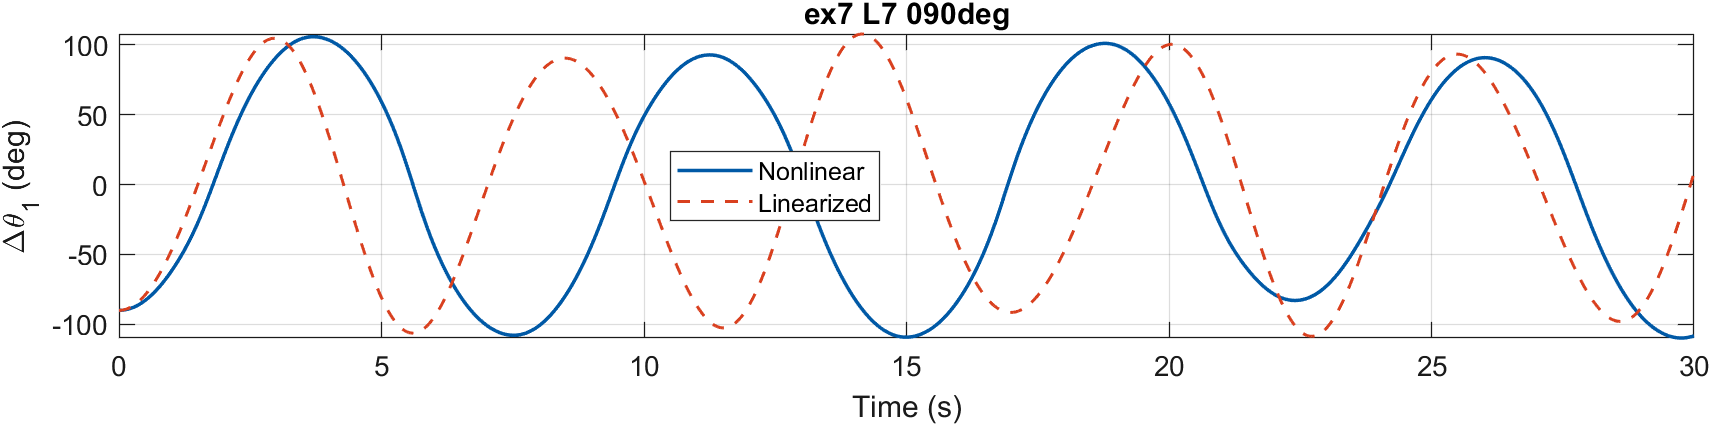
\includegraphics[width=0.94\linewidth]{figures/ex7_L7_090deg_theta1.png}
\caption{$\Delta\theta_1$: nonlinear and linearized time histories.}
\end{figure}
\begin{figure}[!ht]
\centering
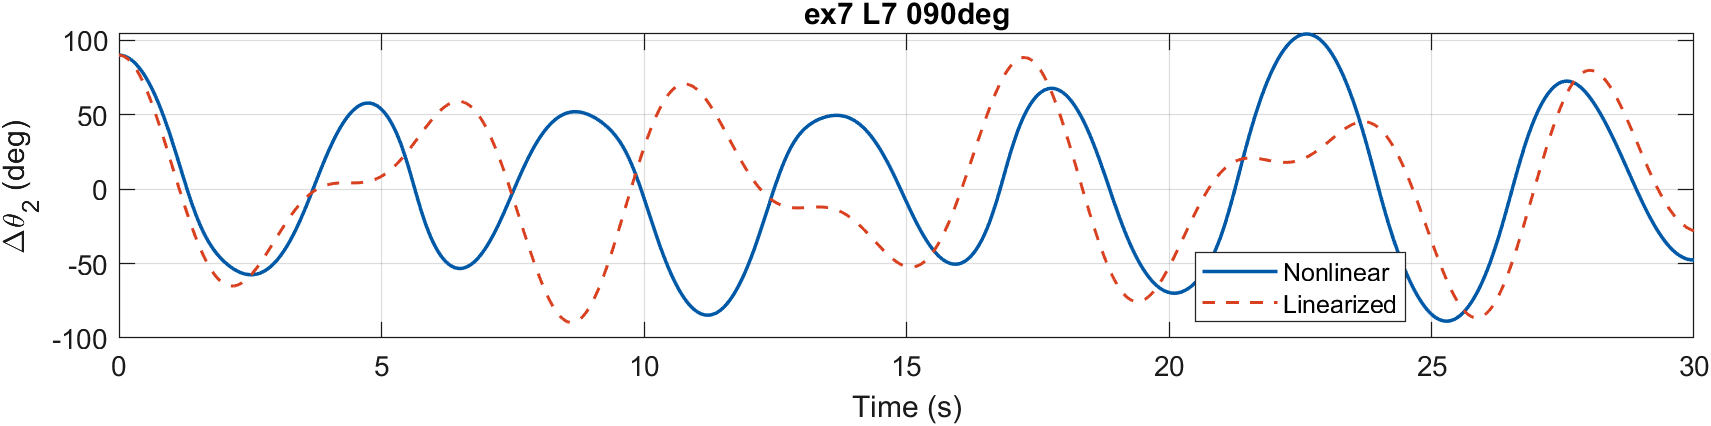
\includegraphics[width=0.94\linewidth]{figures/ex7_L7_090deg_theta2.png}
\caption{$\Delta\theta_2$: nonlinear and linearized time histories.}
\end{figure}

\textbf{MATLAB code for L7, $\pm90^\circ$:}
The following case-specific block uses the common local functions \texttt{simulate\_case} and \texttt{export\_case} listed in the source appendix.
\begin{lstlisting}
p = [2 1 1 1 0.5 1]; % [m0 m1 m2 l1 l2 g]
model = cart_pendulum_model(p, 1);
alpha = 90; % degrees
z0 = [0; -deg2rad(alpha); deg2rad(alpha); 0; 0; 0];
options = odeset('RelTol',1e-10,'AbsTol',1e-12,'MaxStep',0.02);
r = simulate_case(model, z0, 30, 'ex7_L7_090deg', options);
export_case(r, outputDir, rootDir);
\end{lstlisting}

\clearpage
\subsection*{\texttt{ex7\_L7\_180deg}}
Initial deviation $z(0)$ (radians for angles, SI units otherwise):
\begin{center}\scriptsize\texttt{[0, -3.141593, 3.141593, 0, 0, 0]}\end{center}
$x^e=[0,0,0,0,0,0]^T$, $x(0)=x^e+z(0)$.
\begin{figure}[!ht]
\centering
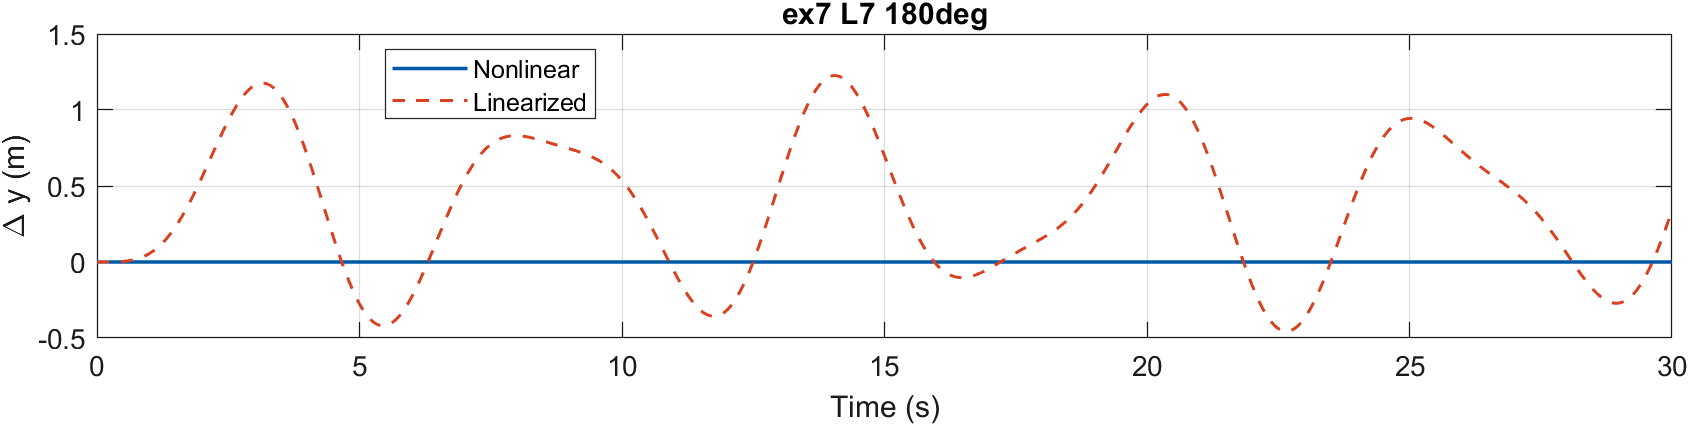
\includegraphics[width=0.94\linewidth]{figures/ex7_L7_180deg_y.png}
\caption{$\Delta y$: nonlinear and linearized time histories.}
\end{figure}
\begin{figure}[!ht]
\centering
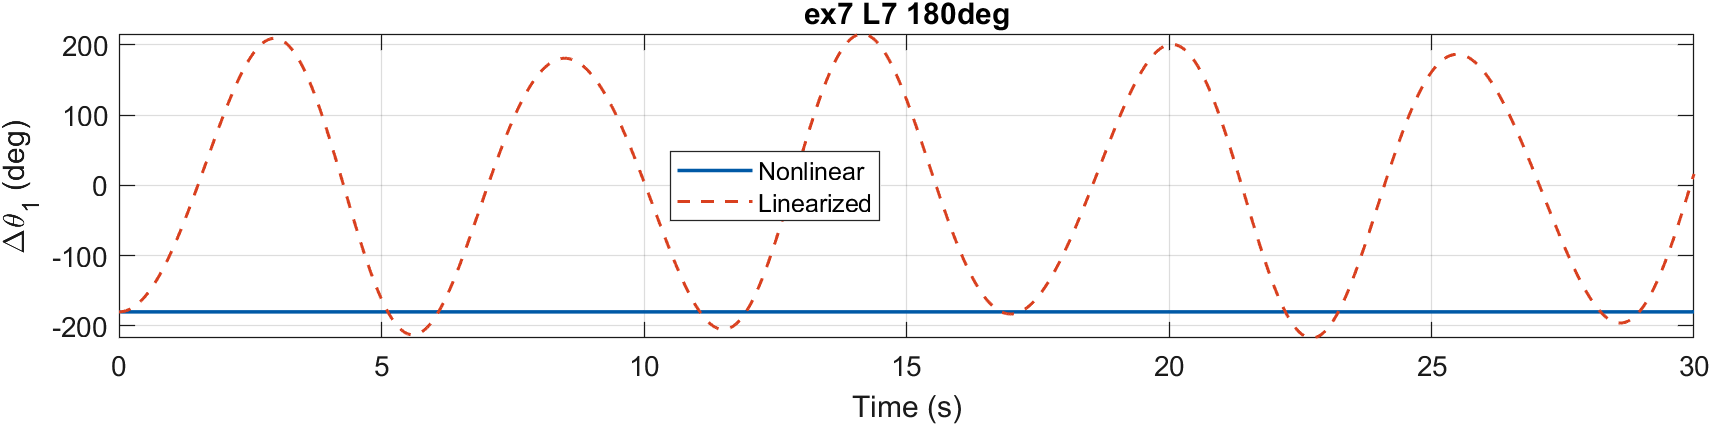
\includegraphics[width=0.94\linewidth]{figures/ex7_L7_180deg_theta1.png}
\caption{$\Delta\theta_1$: nonlinear and linearized time histories.}
\end{figure}
\begin{figure}[!ht]
\centering
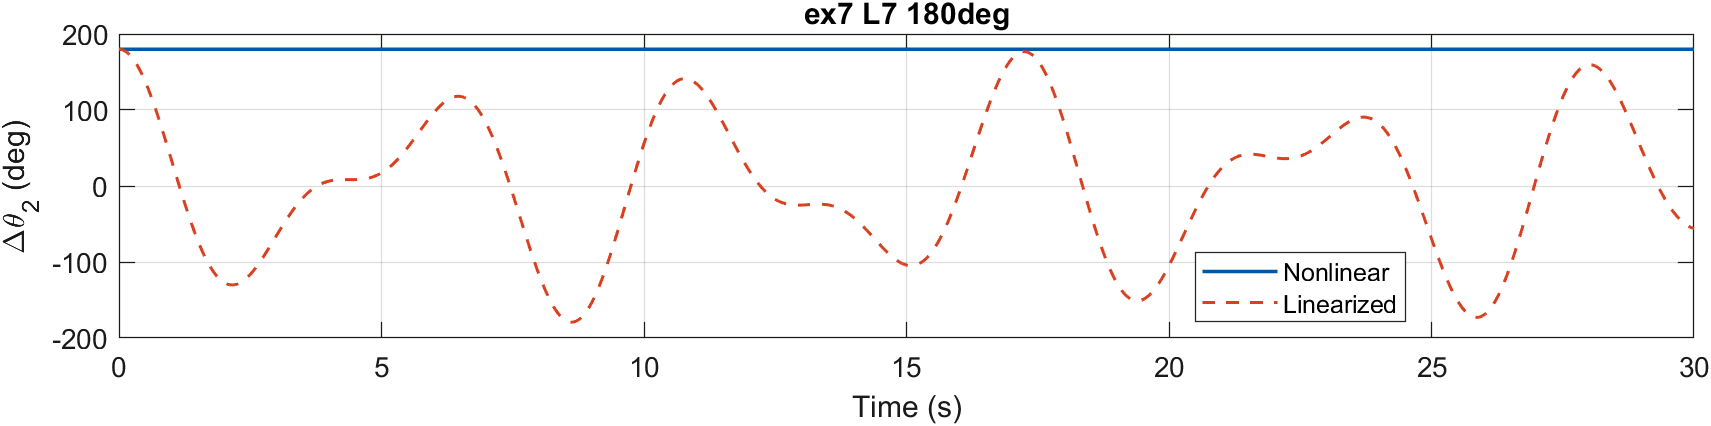
\includegraphics[width=0.94\linewidth]{figures/ex7_L7_180deg_theta2.png}
\caption{$\Delta\theta_2$: nonlinear and linearized time histories.}
\end{figure}

\clearpage
\subsection*{\texttt{ex7\_L8\_001deg}}
Initial deviation $z(0)$ (radians for angles, SI units otherwise):
\begin{center}\scriptsize\texttt{[0, -0.01745329, 0.01745329, 0, 0, 0]}\end{center}
$x^e=[0,3.141593,3.141593,0,0,0]^T$, $x(0)=x^e+z(0)$.
\begin{figure}[!ht]
\centering
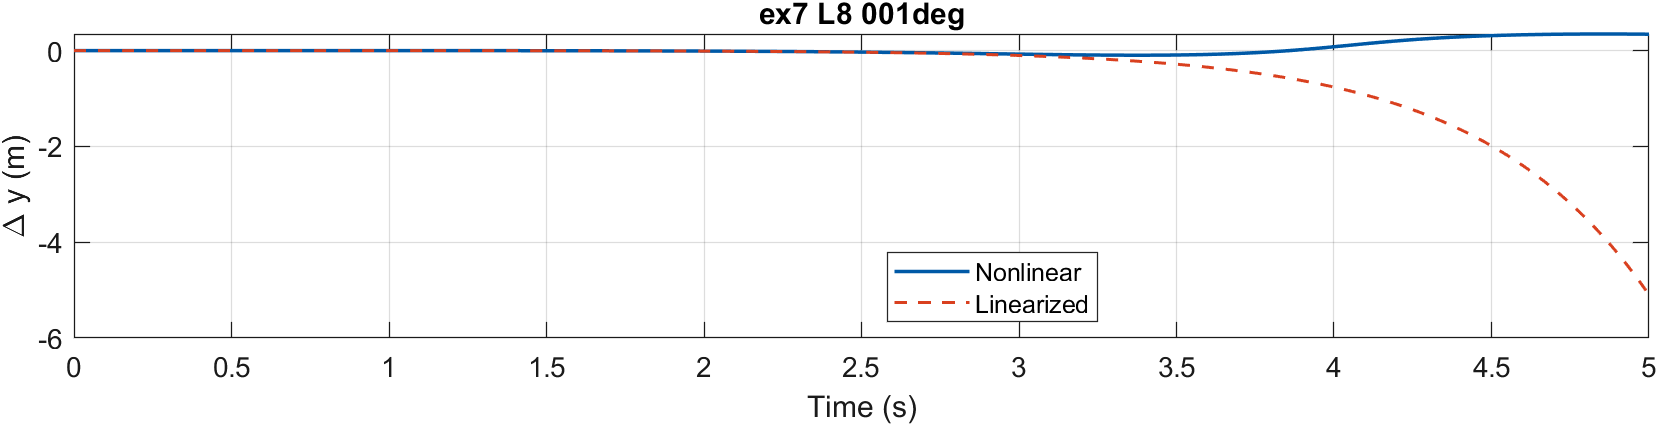
\includegraphics[width=0.94\linewidth]{figures/ex7_L8_001deg_y.png}
\caption{$\Delta y$: nonlinear and linearized time histories.}
\end{figure}
\begin{figure}[!ht]
\centering
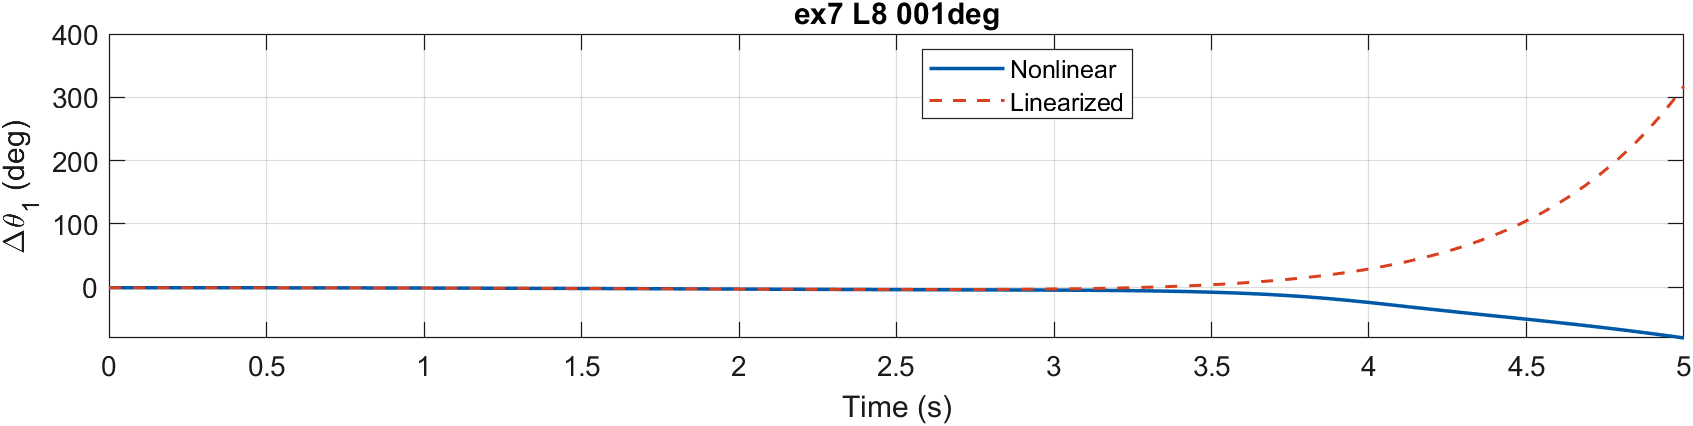
\includegraphics[width=0.94\linewidth]{figures/ex7_L8_001deg_theta1.png}
\caption{$\Delta\theta_1$: nonlinear and linearized time histories.}
\end{figure}
\begin{figure}[!ht]
\centering
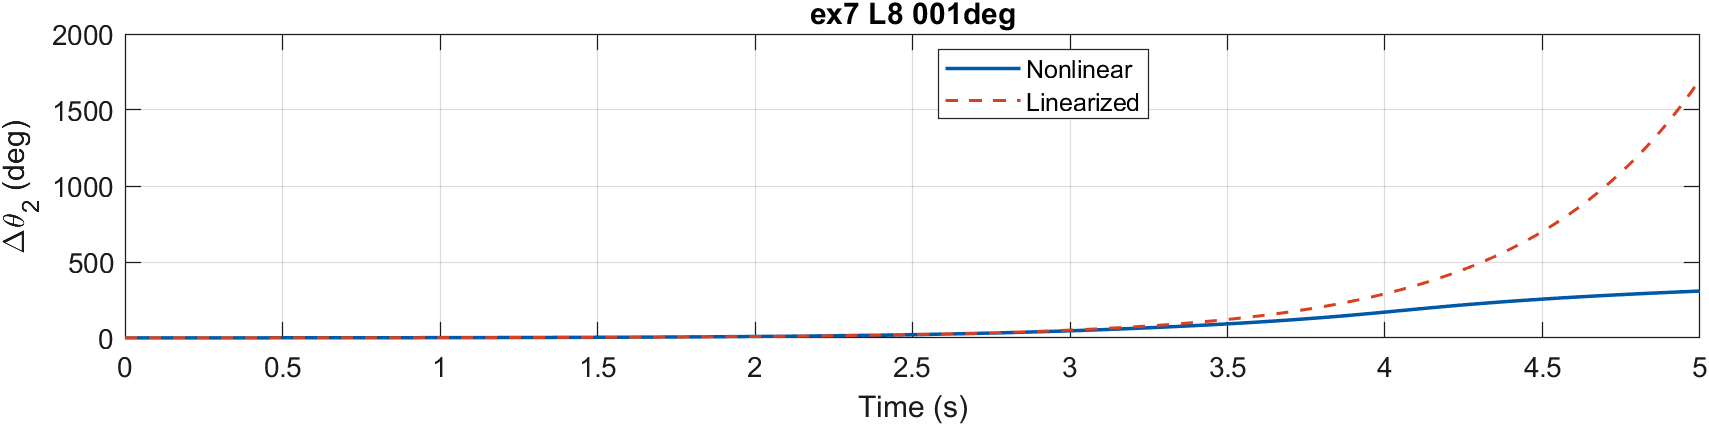
\includegraphics[width=0.94\linewidth]{figures/ex7_L8_001deg_theta2.png}
\caption{$\Delta\theta_2$: nonlinear and linearized time histories.}
\end{figure}

